\documentclass[12pt,a4paper]{article}
\usepackage{times}
\usepackage{durhampaper}
\usepackage{harvard}
\usepackage{graphicx}

\usepackage{multicol}
\usepackage{subfig}

\citationmode{abbr}
\bibliographystyle{agsm}

\title{Predicting medium-term train delays using machine learning}
\student{Dominic White}
\supervisor{Noura Al-Mouyabed}
\degree{BSc Computer Science}

\date{}

\begin{document}

\maketitle

\begin{abstract}

\subsection{Context / Background}

Trains are one of the most popular forms of public transport. The perceived likelihood and severity of train delays is a turn-off for many consumers, and so a system predicting train delays in the medium-term would improve both customer satisfaction and operating profits. There are currently no solutions to this problem in the literature, nor in practice, although extensive research has been carried out into real-time delay prediction.

\subsection{Aims}

The aims of this project are twofold. The primary aim is to identify a suitable binary classification model for predicting medium-term train delays. The secondary, supporting aim is to develop a new train delay dataset to train this model on, as there are none publicly available. 

\subsection{Method}

Using historical schedule data, movement data, location data, and weather data from a variety of sources, a high-quality dataset is constructed for use in machine learning. A variety of classification models are trained and tested, and the best-performing is optimised. The effect of including exogenous weather data is investigated.

\subsection{Results}

An entirely new high-quality dataset has been constructed, comprising $5.2$ million rows and $23$ columns. Of the classification models tested, a random forest achieved the greatest $F_1$-measure of $0.76$. Evaluation using repeated stratified $6-$fold cross validation resulted in a $ROC_{AUC}$ of $0.86$. 

\subsection{Conclusions}

This project explores a relatively unstudied area in train delay prediction. The dataset developed is novel and high-quality, and may prove of use to other researchers. The developed random forest performed well, and together they form a solid foundation for future work in this area.

\end{abstract}

\begin{keywords}
Machine learning, train delay, delay prediction, extract-transform-load, etl, classification, regression
\end{keywords}

\clearpage
\section{Introduction}

$1.76$ billion rail journeys were made in the 2018 - 2019 financial year\footnote{https://dataportal.orr.gov.uk/statistics/usage/passenger-rail-usage/}. Of these journeys, approximately $12.2$\% were delayed by more than 5 minutes. Train delays impose a huge cost on passengers and operators by contributing to the inefficiency of train operations (Van Oort, 2011). In 2006 – 07, for example, delays cost a minimum of £1 billion in terms of time lost to passengers \cite{nao_2008}. Furthermore, under a scheme known as ‘Delay Repay’, train operating companies (TOCs) are automatically obliged to refund $50\%$ of the cost of passengers’ tickets if a train is between 30 – 60 minutes late and $100\%$ if it is more than 60 minutes late. $4.6$ million fares were repaid in 2018 - 2019.

So it is no understatement to say that train delay is a serious problem. The issue is compounded for passengers, who tend to perceive punctuality as worse than it is for three reasons: passengers tend to recall delayed trains over punctual trains; more passengers travel on late trains than punctual trains (as passengers accumulate while waiting); and operators avoid early running, so late trains are not balanced out by early trains \cite[p.~130]{harris_godward_1992}. Furthermore, passengers expect trains to run on time as TOCs are considered to be in greater control of their environment.

This mismatch in perception places great importance on reducing the impact of delays on passengers. So: what if passengers could know in advance whether or not a train would be delayed? The aim of this project is not to answer this questions, but to see whether doing so is possible: can train delays be predicted in advance? 

Systems already exist for predicting real-time train delay; the problem is well-studied. The majority are analytical \cite{oneto_et_al_2016}. Such models are online, i.e. updated as information on train movements becomes periodically available. At the other end of the spectrum is the optimisation problem of train scheduling, which is also very well studied. Between the two extremes lies is a poorly-defined region, the medium-term timeframe, neither online nor offline, lower-bounded by the availability of forecasts of exogenous data and upper-bounded by the times trains depart their origins. This is the timeframe this project focuses on. Knowing that a train will be delayed while on it is of little help to most passengers, but knowing it will be a week in advance is. 

This project will explore data-driven models, which have recently been gaining traction in the field. Rete Ferroviaria Italiana (RFI), the Italian railway manager, uses a (real-time) model \cite{oneto_et_al_2016}; Deutsche Bahn (DB), a German railway operator, recently commissioned a comprehensive study into a (real-time) model suitable for their network \cite{lessan_fu_wen_2019}. This work aims to develop both a train delay dataset and a data-driven binary classification model to see whether medium-term train delays can be predicted.

\subsection{Background}

Although precise terminology differs, the literature agrees that there are two principal classes of delay \cite{olsson_haugland_2004}: primary (exogenous) and secondary (knock-on, consecutive). A primary delay is caused by external stochastic disturbances \cite{oneto_et_al_2016}, of which there are many potential causes \cite{berger_et_al_2011,milinkovic_et_al_2013}. They may be classified into three categories: infrastructure, weather, engineering, and a catch-all (other). This is presented in Table~\ref{table:primary_delay}. Of the delays in 2006 - 2007, $42$\% were caused by infrastructure faults, $38$\% by TOCs, and the remaining $20$\% by events such as adverse weather, fatalities and vandalism. 

\begin{table}[]
\centering
\caption{Causes of primary delays}
\label{table:primary_delay}
\begin{tabular}{|l|l|}
\hline
\textbf{Class} & \textbf{Causes of delay}                                      \\ \hline
Infrastructure & Signals and point failures; malfunctioning equipment          \\ \hline
Weather        & Severe heat; flooding; landslips; leaves; snow and ice        \\ \hline
Engineering    & Scheduled maintenance; repairs                                \\ \hline
Other          & Prolonged alighting and boarding times; fatalities; accidents \\ \hline
\end{tabular}
\end{table}

A secondary delay is generated by operational conflict (Cerreto \textit{et al.}, 2016). Primary delays induce a cascade of secondary delays of other trains, which must wait for tracks to be clear, crews to be in the right place, platforms available, and so on. This is visualised in Figure~\ref{fig:delay_propagation}. Predicting secondary delays is very difficult; it is the source of the complexity of real-time models. As Lessan \textit{et al.} (Lessan \textit{et al.}, 2019) note, some secondary delay factors are predictable and controllable: most are neither. This project therefore focuses on predicting primary delays, which depends on exogenous data. 

\begin{figure}[h!]
    \centering
    \subfloat[02:48]{{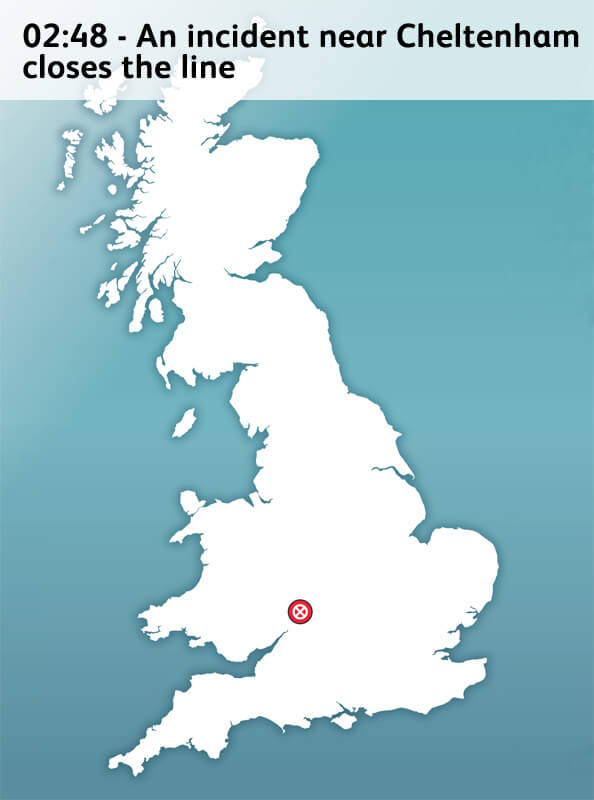
\includegraphics[width=3.5cm]{images/Knock-on-delays-1.jpg} }}
    \quad
    \subfloat[08:48]{{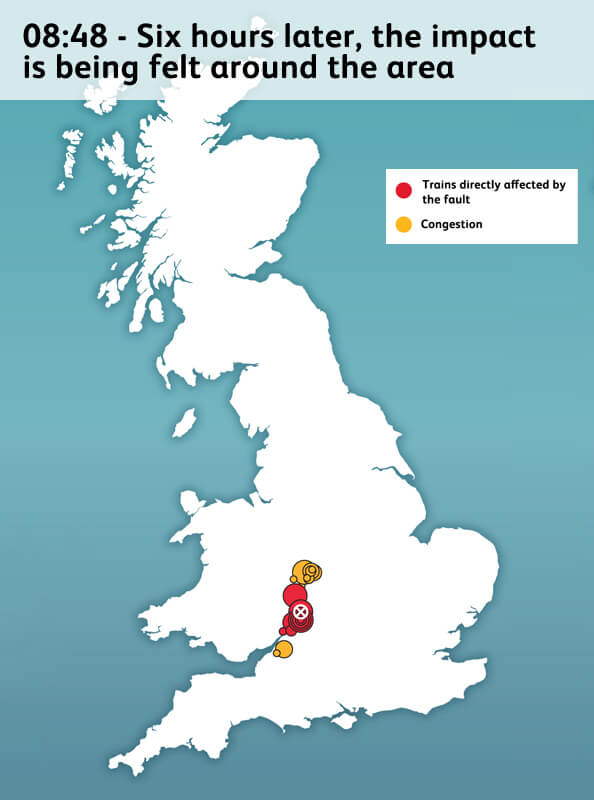
\includegraphics[width=3.5cm]{images/Knock-on-delays-2.jpg} }}
    \quad
    \subfloat[15:18]{{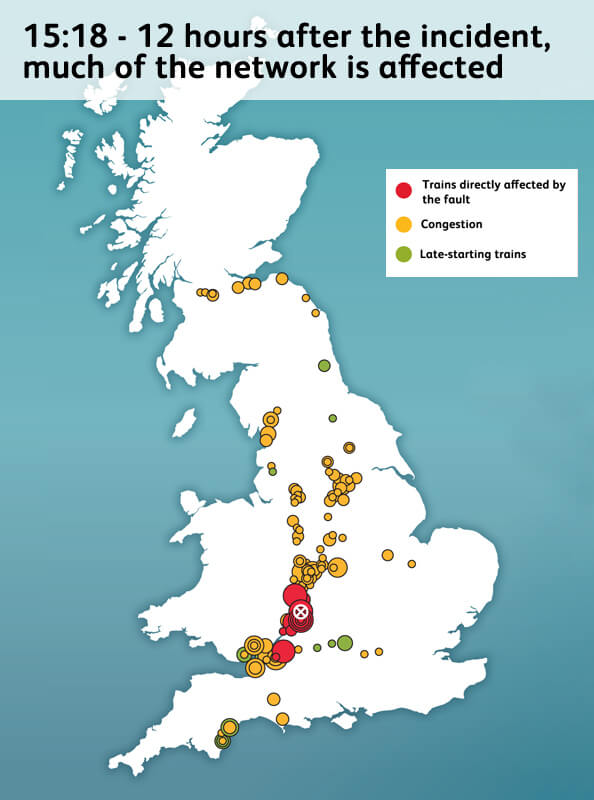
\includegraphics[width=3.5cm]{images/Knock-on-delays-3.jpg} }}
    \quad
    \subfloat[22:48]{{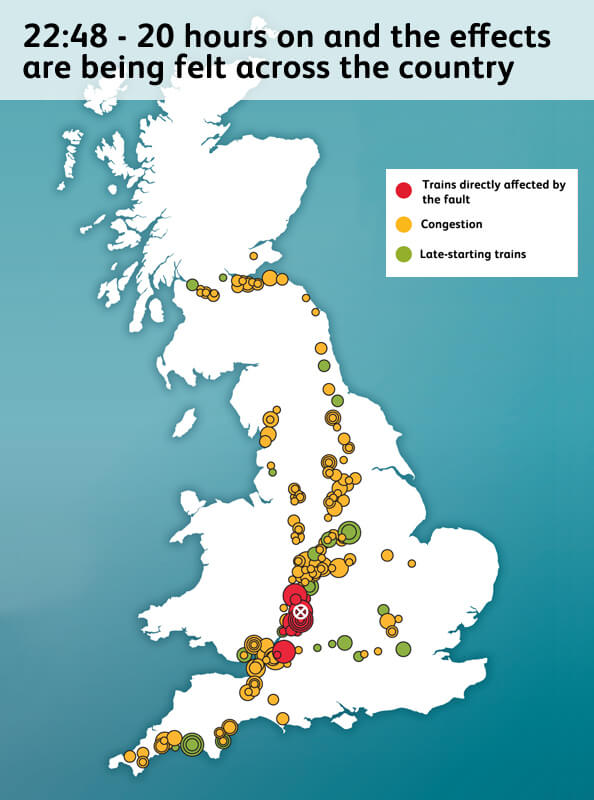
\includegraphics[width=3.5cm]{images/Knock-on-delays-4.jpg} }}
    \caption{A visualisation of delay propagation. A single incident at 02:48 causes congestions, delays and cancellations across most of the country for the next $24$ hours. Red dots are trains directly affected by the fault; yellow, congestion; green, late-running trains.}
    \label{fig:delay_propagation}
\end{figure}

Data is exogenous if it is independent of other input data but the output is dependent upon it. In the context of primary delay prediction, the more of the causes of primary delay that can be incorporated into a model, the better it will perform. Models tend to use a combination of infrastructure \cite{markovic_et_al_2015,milinkovic_et_al_2013,lessan_et_al_2019}, weather (Oneto \textit{et al.}, 2016; Wang and Zhang, 2018; Oneto \textit{et al.}, 2017; Lessan \textit{et al.}, 2019), expert opinions (Markovic\textit{et al.}, 2015; Oneto \textit{et al.}, 2019) and engineering work (Lessan \textit{et al.} 2019). Oneto \textit{et al.} (2017) also recommends using information about passenger flows and about railway asset conditions.  Where directly relevant exogenous data is not available, it is possible to use proxies (Harris, 1992), such as: 

\begin{itemize}
	\item{train length (as a proxy for the number of doors to manage, and passenger demand)}
	\item{distance covered (as a proxy for the likelihood of encountering track defects and other technical / operational problems)}
	\item{the previous number of stops (as a proxy for cumulative delay resulting from passengers alighting and boarding)}
	\item{the age of the motive power unit (as a proxy for reliability; it is industry-held fact that a motive unit’s reliability declines after 20 years)}
	\item{track occupation (as a proxy for capacity utilisation the railway, and thus the likelihood of delays propagating)}
\end{itemize}

\subsection{Objectives}

The research question proposed is: \textit{can medium-term train delays be predicted}? To address this question, the objectives for this project were divided into three categories: minimum, intermediate, and advanced. 

The minimum objective of this project is to construct a high-quality dataset incorporating a variety of exogenous data. The purpose of this objective is twofold. It is, first and foremost, a prerequisite for machine learning. Secondly, however, it will establish a strong understanding of the data itself, informing feature engineering in the intermediate and advanced objectives. There are few objective criteria for what makes a good dataset, save that it ought to be clean, logically structured, and complete, and fields included relevant. 

The intermediate objective is to develop a binary classification model to predict whether a train will be delayed. A variety of classification models will be selected, with selection informed by a literature review, then tested. The best-performing model will further tuned. With no benchmark for comparison, any accuracy target would be arbitrary; so this model is expected to be better than a random guess. 

The advanced objective is to build upon the intermediate objective by developing a regression model to predict by how much a train will be delayed. This problem is markedly harder than classification, and so performance is expected to be corresponding worse too. As before, the best-performing model will be extensively fine-tuned.

\section{Related Work}
\label{section:related_work}

In the section, we present work related to our research question: \textit{Can medium-term train delays be predicted?}. Although there has been significant academic effort into producing real-time TDP systems, research on medium-term TDP is rather sparse. Fortunately, there is considerable overlap between the two timeframes. Solutions to the problem of real-time TDP use a variety of machine learning regression models, with the field tending towards ensembles / hybrids  and random forests. The inclusion of exogenous data pertaining to weather and infrastructure is also popular.  There are many classifications of TDP models, based on scope, model type, and solution methods \cite{markovic_et_al_2015}. Generally, approaches may be divided using two axes: whether they are offline or online, and whether they use analytical or data-driven models. As this project is concerned with latter, the former is discussed only briefly. Online models are updated with new data as it comes available; data-driven models are trained using historical data.

\subsection{Analytical approaches}

An analytical model is “primarily quantitative or computational in nature and represents the system in terms of a set of mathematical equations that specify parametric relationships and their associated parameter values as a function of time, space, and/or other system parameters” \cite{friedenthal_moore_steiner_2012}. Current state-of-the-art train delay prediction systems use analytical models \cite{oneto_et_al_2016}: “static rules, built by experts on railway infrastructure, and based on classical univariate statistics”.

Simplistic early models, such as those developed by \cite{frank_1966} make overly restrictive assumptions about railway operations, e.g. no overtakes are allowed, departure times are uniformly distributed, and that the speed of each train is unique and constant. Subsequent work in this area has largely relaxed these assumptions by including factors such as overtakes, different speeds, priority systems, and uncertainties associated with train departure time \cite{petersen_1974,chen_harker_1990}. Further models have become increasingly advanced, incorporating stochastic approximation \cite{carey_kwiecinski_1994}, and the impacts of dispatching strategies on train delays and passenger waiting time. The current state-of-the-art is likely \cite{berger_et_al_2011}, whose model is currently used by DB.

Much work has also been done by Kecman and Corman (Kecman, Corman, and Meng, 2015; Kecman, Corman, Peterson, and Joborn, 2015; Corman and Kecman; 2018) which blurs the line between analytical models and data-driven models. The authors use stochastic models based on Bayesian networks and trained on historical data to predict delays, with considerable success.

However, there is a fundamental limit on the complexity of such models, and as the field of machine learning has matured, the applicability of data-driven models to TDP has been increasingly well explored. 

\subsection{Online / dynamic data-driven approaches}

Most real-time TDP systems are online. The first comprehensive attempt at developing a TDP system was made by Oneto et al. (2016). Subsequent papers (Oneto et al., 2017; Oneto et al., 2019) have expanded proposed models in scope and performance.
The authors consider a rail network a graph, where nodes represent checkpoints and edges tracks connecting them. A train follows an itinerary composed of $N_c$ checkpoints characterised by an origin, a terminus, and intermediate locations such as stops and transits. A schedule is modelled as a time series forecast problem, with performance at previous checkpoints used to predict performance at subsequent checkpoints. A model for each train is trained using historical delay data. The authors tested random forests (RF), extreme learning machines (ELM), and kernel methods (KM) and found that their RF performed twice as well as current state-of-the-art TDP systems. The inclusion of weather further improved accuracy by approximately 10\%. Their model was very computationally expensive, however, requiring approximately 600,000 models to be trained daily across the entire rail network. 

The authors then generalise their work to produce a dynamic data-driven TDP system (Oneto et al., 2017), with performance tuned using thresholdout, which reduces overfitting. They compare the performance of two implementations of shallow and deep ELMs. 
This work laid the groundwork for their most recent paper, which combines an experience-based model (EBM) and multiple RF into a hybrid model (HM) (Oneto et al., 2019). The EBM uses operators’ knowledge and experience of the network to inform features. As Martin (2016) notes, in real-world train operations, delay prediction relies heavily on the experience and intuition of a local dispatcher, rather than a network-work computational instrument. The HM is a decision tree where each leaf is a RF. Trains are directed to the appropriate RF by similarity, eliminating the need for a model for every train. A new leaf is added each time a new train is seen that belongs to a previously unexplored branch of the decision tree. The RF regressor in the leaf is trained based on all the past train movements in that leaf. This model has several unique features. Trains older than 3 months are ‘forgotten’, to keep the size of the model constrained. Furthermore, this model naturally handles the mercurial nature of train schedules, which are both released periodically and revised constantly. The model required only 10 days’ of data after a new schedule comes into effect to reach optimal accuracy, with excellent performance also noted for outliers. The HM offers the best trade-off between accuracy and computational requirements, with superior results to all current models. 

A similarly impressive model was developed by Lessan et al. (Lessan et al., 2019), working closely with Deutsche Bahn (DB). The authors used 3.25 years’ of data from DB and incorporated a wide range of exogenous data, with approximately 350 features for operational (i.e. currently running) trains and 70 for non-operational trains. The authors tested support vector regression (SVR) but settled on RF. Three models were used for operational trains: an online RF, mesoscopic simulation, and kernel regression. Two were used for non-operational trains: an offline RF and mesoscopic simulation. The authors found an accuracy of over 80\% in predictions within a 60-minute horizon, a considerable improvement in real-time forecasts, but found that beyond that horizon predictions were only marginally better than the schedule. 

\subsection{Offline / static data-driven approaches}

Static models are not updated with data as it comes available. Early attempts used simple neural networks (Peters et al., 2005) and were essentially proofs-of-concept. The use of neural networks was further investigated by Yaghini et al. (Yaghini et al., 2011) using data from Iranian Railways to predict the late arrival of passenger trains. Their model performed better to alternatives such as decision trees and logistic regression. The authors also tested the impact of various encoding schemes. 

Subsequent work is largely exploratory, with no clear direction as described in the previous section. Papers investigate a wide variety of models, such as fuzzy Petri nets (FPNs) (Milinkovic et al., 2013), support vector regression (SVM) (Markovic et al., 2015), logistic regression (Wang and Work, 2015) and gradient-boosted random forests (Wang and Zhang, 2019).

FPNs are mathematical modelling tools used to analyse and simulate concurrent systems (Murata, 1989). The authors explored two separate FPNs. In the first, expert knowledge was used to define fuzzy sets and rules. In the second, an Adaptive Network Fuzzy Inference System (ANFIS) was trained on historical delay data and then replicated in an FPN. Both were then tested with real data from a Belgrade station node. The ANFIS-FPN produced results within 5\% of actual delay values for a subset of the data; slightly worse performance was observed for the expert-defined FPN.

Markovic et al. (Markovic et al., 2015) presented the first use of SVM. They found it outperformed artificial neural networks.  Data for the analysis was again collected from Serbian Railways. The paper used the expert opinions of dispatchers to estimate the likelihood of multiple factors along a rail line, such as single-tracking, junctions, or the number of stations, causing a delay, using the Delphi method to obtain a final estimate. A strong correlation was found between expert opinions and train delays. The focus was on developing a functional relationship between delays and infrastructure so the effect of infrastructure improvements on delays can be predicted and valued.  

Wang and Work (Wang and Work, 2015) used data from Amtrak to develop two vector autoregression models: one offline, the other online. The offline model improved the RMSE of predicted delays by 12\%; the online model, by 60\%. Vector autoregression is a model that capture the linear interdependence between multiple time series (i.e. each train). 

Wang and Zhang (Wang and Zhang, 2019) present a relatively simple gradient-boosted regression trees (GBRT) model. The model was trained on a three-month dataset of weather, train delay, and train schedule records. Their model can make predictions up to 10 days’ in advance, the limit of the weather forecast system used, but performed poorly, which the authors attribute to the limited size of their dataset. This paper most closely resembles the objectives of this project. 

\clearpage
\section{Solution}
\label{section:solution}

In this solution we present our solution to constructing a dataset and identifying a suitable binary classification model. The \verb|Python| programming language was used throughout, with \verb|NumPy| for numerical operations, \verb|Pandas| for data manipulation and analysis, \verb|scikit-learn| for machine learning, and \verb|Matplotlib| for graphing. 

\subsection{Dataset construction: the Extract-Transform-Load (ETL) pipeline}

Central to the importance of machine learning is a high-quality labelled dataset. Unfortunately, there are no publicly available datasets for train delay. Correspondence between authors of previous papers \cite{yaghini_et_al_2013,wang_zhang_2019} proved unfruitful, so it was necessary to construct a new dataset, which became the minimum objective of this project. Dataset construction is a complex task. It falls under the purview of the Extract-Transform-Load (ETL) pipeline\footnote{Sometimes a different order is used: Extract-Load-Transform (ELT). The sole difference is where the transformation stage takes place. The distinction is largely academic here, so ETL is used throughout.}. This pipeline extracts data from sources, transforms them into a usable format, and loads them into storage for future operations. It is a very time-consuming task: “it is not uncommon for a project team to spend as much as 50\% to 70\% of project effort on ETL functions” \cite[p.~284]{ponniah_2010}. This proved the case with this project, so we dedicate considerable space to explaining each stage in the pipeline, and how it was realised in the context of this dissertation.

First, we identified suitable data sources for the train data itself (schedules, location, and movement) and the four classes of primary delay (weather, infrastructure, passenger, and engineering). The UK rail infrastructure manager Network Rail (NR) opend its feeds\footnote{https://www.networkrail.co.uk/who-we-are/transparency-and-ethics/transparency/open-data-feeds/} to developer usage in $2011$; they are presented in Table~\ref{table:nr_feeds}.

\begin{table}[htb]
\centering
\caption{Network Rail data feeds and their use in this project. I = investigated, U = used, N = not used.}
\label{table:nr_feeds}
\begin{tabular}{|l|p{8cm}|p{2cm}|c|}
\hline
\textbf{Acronym} & \textbf{Description} & \textbf{Frequency} & \multicolumn{1}{l|}{\textbf{Usage}} \\ \hline
BPLAN & Train planning data, including locations and sectional running times. & Twice a year & I \\ \hline
CORPUS & Location reference data. & Monthly & U \\ \hline
MOVEMENT & Train positioning and movement event data. & Real-time & U \\ \hline
RTPPM & Performance of trains against the timetable, measured as the percentage of trains arriving at their destination on-time. & Once a minute         & N \\ \hline
SCHEDULE         & Daily extracts and updates of train schedules from the Integrated Train Planning System (ITPS).                          & Overnight each night  & U                                       \\ \hline
SMART            & Train describer berth offset data used for train reporting.                                                              & Monthly               & N                                       \\ \hline
TD               & Train positioning data at a signalling berth level.                                                                      & Real-time             & N                                       \\ \hline
TSR              & Details of temporary reductions in permissible speed across the rail network.                                            & Once a week on Friday & I                                       \\ \hline
VSTP             & Train schedules created via the VSTP process                                                                             & Real-time             & I                                       \\ \hline
\end{tabular}
\end{table}

\subsubsection{Schedules: SCHEDULE}

Schedules are available as CIF files. A full CIF – a database snapshot – is released every Friday morning, with update CIFs released every morning. Each update must be applied to the latest full CIF to maintain a correct database. Each file contains train schedules, metadata, and associations.

\subsubsection{Movement: TD, TRUST, and Darwin}

The TD feed provides information about the position of trains through a network of berths. A berth usually represents a signal. TD was discarded as too low-level for this project. There are two movement systems in use: Train Running Under System TOPS (TRUST) and Darwin. TRUST is a NR system used for monitoring the progress of trains and tracking delays in the UK. Darwin uses both TRUST and TD for real-time data, and also incorporates Darwin workstations, Customer Information Systems (CIS), and internal messaging systems.

TD feeds into TRUST, and TRUST into DARWIN. Darwin provides more comprehensive information. While the objectives of this project were being defined, it was undecided whether to focus on real-time or medium-term train delays. Real-time would have necessitated the use of Darwin, whereas medium-term could have used either. To keep options open, Darwin was therefore used. Darwin messages contain a lot of extraneous information, but fundamentally each movement message contains a timestamp and a location, either a STANOX or TIPLOC. Both CORPUS and NaPTAN are therefore necessary to ensure a message can be geolocated.

\subsubsection{Location: CORPUS (and NaPTAN)}

CORPUS is used in conjunction with the National Public Transport Access Node (NaPTAN) database, a nationwide system for uniquely identifying all points of access (nodes) to public transport in the UK. Only rail stations are, naturally, of concern here. A large variety of codes are used to refer to locations in the UK rail network; they are presented in Table~\ref{table:codes}.

\begin{table}[h!]
\centering
\caption{UK rail network location codes.}
\label{table:codes}
\begin{tabular}{|p{2.5cm}|c|c|p{8cm}|}
\hline
\textbf{}          & \multicolumn{1}{l|}{\textbf{CORPUS}} & \multicolumn{1}{l|}{\textbf{NaPTAN}} & \textbf{Description}                                                                                                                                                                \\ \hline
STANOX             & Y                                    &                                      & Station Number. First two digits are the geographic area. Can refer to non-station locations such as sidings and junctions. Numbers run broadly north-to-south.                     \\ \hline
UIC                & Y                                    &                                      &                                                                                                                                                                                     \\ \hline
CRS / NRS / 3ALPHA & Y                                    & Y                                    & Used primarily to identify stations and on seat reservation labels.                                                                                                                 \\ \hline
TIPLOC             & Y                                    & Y                                    & Timing Point Location. Relates to points used in deriving train schedules. A station often has multiple TIPLOCs if it consists of  multiple groups of platforms on different lines. \\ \hline
NLC                & Y                                    &                                      & National  Location Code. Identifies locations on the railway. Used for retailing and accounting purposes.                                                                           \\ \hline
NLCDESC            & Y                                    &                                      & A description of the NLC.                                                                                                                                                           \\ \hline
NLCDESC16          & Y                                    &                                      & A description of the NLC.                                                                                                                                                           \\ \hline
ATCO               &                                      & Y                                    &                                                                                                                                                                                     \\ \hline
EASTING, NORTHING  &                                      & Y                                    & Geographic Cartesian coordinates for a point. Uses EPSG:27700\footnote{https://epsg.io/27700}, the British National Grid / Ordnance Survey system.                                                                  \\ \hline
NAME               &                                      & Y                                    & The name of the location.                                                                                                                                                           \\ \hline
\end{tabular}
\end{table}

\subsubsection{Weather: MIDAS, CEDA, and Datapoint}

The primary source of weather data is the Met Office Integrated Data Archive System (MIDAS). MIDAS is a database of land and marine surface observations, collected from 1853 to the present day, by the Met Office station network. MIDAS offers several datasets. The most comprehensive is the Hourly Weather Observation Data, which contains meteorological values measured on an hourly time scale. These observations include 104 fields , though many are for quality control, or too specific to necessitate inclusion. Station data is available from the Centre for Environmental Data Analysis (CEDA). Each station is geolocated by latitude and longitude. 

For this project to be useable, trained models must be applicable to unseen data. Unseen train data are simply train schedules. Unseen weather data are forecasts. Forecasts are available from Met Office Datapoint, a service allow access to freely available Met Office data feeds. They may be obtained as 3-hourly site-specific forecasts up to 5 days’ in advance. There are over 5,000 UK forecast sites. There are 10 forecast available fields. 

\subsubsection{Infrastructure: BPLAN and the Train Planning Network Model}

The Train Planning Network Model is used by the Integrated Train Planning System (ITPS). Unfortunately, we were unable to integrate either of these datasets, as there was simply too little documentation.

\subsubsection{Engineering: TSR}

TSR provides proxy details of engineering works. It was unfortunately not archived in the repository used for the rest of the NR data, and so we could not make sure of it.

\subsection{Extraction}

Extraction is the process of collecting data, often from multiple different sources, and moving it to a \textit{staging area}. Some basic validation also takes place at this stage. The extraction process of the each data source is presented in Table~\ref{table:extraction}.

\begin{table}[htb]
\centering
\caption{Extraction methods for each data source}
\label{table:extraction}
\begin{tabular}{|l|p{12cm}|}
\hline
\textbf{Data source} & \textbf{Notes}                                                                                                                                                                                                                                                                                                                                                                                                                                                                                                                                                                                                                                           \\ \hline
Schedule            & Schedule data is available from Peter Hicks’ website . Both full and update extracts are downloaded as gzipped files.                                                                                                                                                                                                                                                                                                                                                                                                                                                                                                                                    \\ \hline
Movement            & Darwin data is also available from Peter Hicks’ website . Each day is a bzip2-compressed tar file containing 1440 files, one for each minute in the day. Each file comprises XML messages. Each minute is extracted in memory and written to one CSV for each day / file.                                                                                                                                                                                                                                                                                                                                                                                \\ \hline
Location            & NaPTAN is available as a zipped CSV from the Department for Transport (DfT). Only the railway nodes are extracted and saved. CORPUS is available from NR as a gzipped JSON. Only the TIPLOC information is extracted and saved.                                                                                                                                                                                                                                                                                                                                                                                                                          \\ \hline
Weather             & Available for download as a CSV file, via FTP from CEDA, though headers must be downloaded separately. Station data is also available from CEDA as a KMZ file\footnote{A KMZ file is a zipped KML (Keyhole Markup Language) file; KML is an XML notation for expressing geographic annotations and visualisations.}. The KMZ file is parsed using pykml and station metadata using BeautifulSoup to produce a CSV. \\ \hline
\end{tabular}
\end{table}

\subsection{Transform}

Transformation is the process of applying a set of functions to extracted data, to clean, map, validate, and consolidate datasets, with the aim of making the data conform to a uniform schema. Typical operations might be mapping NULL to 0, formatting dates, removing duplicate records, converting units, splitting columns into multiple columns (or vice versa), and joining datasets. There is a lot of overlap between transformation and pre-processing, the stage just prior to training. The difference lies in ease of repetition: transformation would, ideally, be performed once, as operations are typically expensive, operating on vast quantities of unstructured and semi-structured data. Pre-processing, using heavily optimised code in NumPy and Pandas, can be iteratively improved.

\subsubsection{Transforming schedules}

Transforming schedules is a difficult task. To retrieve the correct schedule for a given UID on a given day, all schedules with that UID must be retrieved. Those not active on the day in question – as defined by \verb|days_run| – can be discarded, as well as those with a start date in the future. From those remaining, the schedule with the lowest \verb|stp_indicator| is the correct one, in order “C”, “O”, “V”, “P”. “C” is a planned cancellation; “O” is an overlay from STP; “V” is an overlay from LTP; “P” is the permanent base schedule.

As mentioned, an update CIF is released each morning. It contains deletions, amendments, and new schedules, which must be applied to the currently-held schedule database. After each update is applied, the schedules for that day are written to file by filtering those by the criteria above. There is tremendous scope for error. Train scheduling is a very complex problem, and this is reflected in the data formats. Fortunately, full schedules are available weekly, so errors are reset every week. It is likely the bugs in this stage will lead to later problems. 

A CIF file contains 9 types of record: HX (header), BS (schedule metadata), BX (extended schedule metadata), LO (origin), LI (intermediate), LT (terminus), CR (change en route), AA (association) and ZZ (end of file). Of interest are BS, BX, LO, LI, LT. For each BS, a new record is created. A BX may be used to add additional metadata. Each subsequent point (LO, LI, and LT) is used to add new data to the record: the origin, time of departure, number of stops, for instance. 

Two types of record are ignored to reduce complexity: CR (change en route) and AA (associations). An  association represents some dependency between two trains, such as crew or engines. They have the potential to be a rich source of data: is, for instance, a train with more associations more likely to be delayed? Using AAs would necessitate a much more complex model – one that could handle dependencies between trains – rather than the (simpler) tabular format desired. CRs indicate that some metadata contained with BSs changes during a train’s journey. The metadata for a day’s schedules is roughly 60 MB. The route information for a day is roughly 800 MB. Storing the metadata once, rather than merging it onto every location record, significantly reduced space requirements. The other potential solution – checking a database of CRs for every L  - would have incurred significant cost later in the pipeline.  

\subsubsection{Transforming weather}

As mentioned previously, there is a need to map from the MIDAS format to DataPoint format. There are 10 available fields for forecasts, of which only 7 could be meaningfully mapped to equivalent MIDAS fields. For several, this was a simple unit conversion. Boolean masks are used to convert \verb|wind_speed| and \verb|wind_gust| to mph. For visibility and weather type, predefined codes were used to establish a map between the two formats\footnote{https://www.metoffice.gov.uk/services/data/datapoint/code-definitions}. 

\subsubsection{Transforming movement}

Each day of train movements is a file roughly 1.5GB in size. This file also contains a variety of other messages: forecasts, schedules, station messages, alarms, warnings, and so on. The data must be converted into a CSV for usage. It is assumed that no trains runs longer than 24 hours, i.e. there is no train that starts on a given date and ends two days afterward. Each record may have a selection of arrival, departure, and pass times: working, estimated, and public, as well as a lot metadata relating to whether to show certain fields to the public which can be safely discarded. Each train’s information is written to the date it started, and ultimately comprised just five columns: service start date, UID, location, type, and time. It is common for several different messages to refer to the same train movement, a result of Darwin re-reporting movements when updating forecasts. In these instances, duplicates are dropped. If times disagree, the average is taken. 

\subsubsection{Transforming location}

This stage was relatively simple. NaPTAN and CORPUS were merged, and the closest geographical weather station used in the dataset was calculated for future weather look-up. 

\subsection{Load}

Load is the process of storing data in a format accessible for future usage. It was a more complex in this project, involving the merging of the four data classes. Each row should be a train. For every UID in the schedule dataset for a given day, find the matching movement records, append the origin and terminus of each train, and calculate the delay using the value in the schedule values. Finally, use the origin and destination locations to identify the closest weather station, and from there add information on the weather experienced at the start and end of a train’s journey. 

There is plenty of scope for error in this stage, in particular from ‘schedule’ UIDs not in ‘movement’ and mismatching TIPLOCs between the ‘schedule’ and ‘movement’ dataframes. These issues cannot be resolved. They are believed to be the result of two planning processes which generate, or modify, schedules: VSTP and STP. In short, it is possible there exists trains in ‘movement’ with no corresponding metadata in ‘schedule’, corresponding to schedules created by VSTP and STP, and vice versa, corresponding to schedules cancelled by either of the two. 

Two target columns are then constructed using the difference between the scheduled arrival time (STA) and actual arrival time (ATA). The first, whether or not a train is delayed, is used for classification. The second, the amount by which a train is delayed, is used for regression. Erroneous values are also discarded. In about 1\% of records, an error in the ETL pipeline resulted in ATAs a day before STAs. This occurred on a small number of trains that run over two days, which were therefore discarded.

Some element of locality is also likely to improve results. Categorically encoding origin and destination TIPLOCs is impractical, as there are approximately 80,000. Nor is there any structure to their designations. Instead, their corresponding STANOX area is used. There are 89 STANOX areas , proxies for geographical areas.

Dropped columns are mostly IDs, and those used to construct the columns discussed above. The actual time of departure (ATD) must also be dropped, as it could not be known in real-life data ahead of time. Also dropped are three metadata columns with too many NaN values: sleepers, reservations, and branding. 

\subsection{Model selection}
\label{subsection:model_selection}

When searching for candidate models, we looked mainly at those with generally good performance at classification tasks, rather than those identified in Section~\ref{section:related_work}, though there was some overlap \cite{wang_zhang_2019,wang_work_2015}. This is because, as discussed earlier, the majority of research into TDP focuses on the real-time timeframe, not the medium-term, and so are not applicable. As this process is exploratory, we chose a wide range of models. As ensembles have proven popular, we focused on those. We also selected several simple linear models, anticipating poor performance, for comparison. For ease of testing, we only used models available in \verb|scikit-learn|. Eight classifiers were chosen for the initial round: a linear Support Vector Classifier (SVC), a random forest (RF), and a gradient-boosted RF.

\clearpage
\section{Results}

In this section, we present the results of our ETL pipeline, our classification model, and our hyperparameter optimisation. We also discuss the metrics used to analyse results. We trained and tested each of the models identified in Section~\ref{section:solution} (\ref{subsection:model_selection}) on the dataset produced by our ETL pipeline, after some transformations and resampling. We further analysed the best-performing model to identify important features, and subjected it to an hyperparameter optimisation process to improve performance. The experiment environment system specification is outlined in Table~\ref{table:experiment}.

\begin{table}[htb]
\centering
\caption{Experiment environment system specification}
\label{table:experiment}
\begin{tabular}{|l|l|}
\hline
{\bf Component} & {\bf Details}                     \\ \hline
Processor & Intel Core i5-6990K 3.6 GHz \\ \hline
GPU       & NVIDIA GeForce 980 TI 8GB   \\ \hline
RAM       & 32 GB 2400 MHz DIMM         \\ \hline
OS        & Windows 10                  \\ \hline
\end{tabular}
\end{table}

\subsection{ETL}

The output of our ETL pipeline is a single CSV, \verb|1.1 GB| in size, containing approximately $5.2$ million rows and $47$ columns. The dataset contains two target columns, a Boolean \verb|delayed|, for binary classification and a scalar \verb|delay| for regression. Before testing our models, we preprocessed our dataset. We encoded datetime data cyclically, whereby each datetime is split into its constituent parts and each part is converted into two values, one for \verb|sin| and one for \verb|cos|, such that each is encoded as a point on unit circle. For compatibility between different models, we one-hot encoded categorical variables and scaled numeric variables to Gaussian. We later relax this requirement. We also resampled the dataset. Approximately $10\%$ of rows are positive (i.e. delayed). This causes poor performance: a model can learn to always predict negative (i.e. not delayed) to trivially achieve approximately $90$\% accuracy. To remedy this we investigated different ways to balance the dataset, and chose to oversample the minority class (i.e. delayed) using SMOTE \cite{chawla_et_al_2002} and randomly undersample the majority class (i.e. not delayed) to achieve a 50:50 ratio. The final form of our dataset is a $(1178694, 283)$ sparse matrix.

\subsection{Binary classification}

To evaluate our models, we will produce accuracy (Acc), precision (Prec), and recall (Rec) statistics using the number of true positive (TP), true negative (TN), false positive (FP), and false negative (FN) classifications of our models. We also use the $F_\beta$-measure (Eq.~\ref{equation:f_measure}). The $F_\beta$-measure is the weighted harmonic mean of precision and recall, which captures the natural trade-off between them. A $\beta$ of $1$ indicates that Prec and Rec are weighted equally importantly.

\begin{equation}
\label{equation:f_measure}
F_\beta = (1 + \beta) \frac{precision \cdot recall}{\beta^2 \cdot (precision + recall)}
\end{equation}

 We trained each of the models identified in Section~\ref{section:solution} (\ref{subsection:model_selection}) on the same $70\%$ of the dataset. No limits were imposed on memory, CPU usage, or time. Two potential models were discarded for incompatibility with the sparse matrix: GaussianNB and HistGradientBoostingClassifier. We then tested the remaining models on the remaining $30\%$ of the dataset, and computed a number of metrics. The results are displayed in Table~\ref{table:results_explore}.

\begin{table}[htb]
\centering
\caption{A full statistical analysis of each model after training}
\label{table:results_explore}
\begin{tabular}{|p{5cm}|c|c|c|c|}
\hline
\textbf{Model}                  & \multicolumn{1}{l|}{\textbf{Acc}} & \multicolumn{1}{l|}{\textbf{Prec}} & \multicolumn{1}{l|}{\textbf{Rec}} & \multicolumn{1}{l|}{\textbf{$F_1$}} \\ \hline
AdaBoostClassifier              & 0.67                              & 0.62                               & 0.67                              & 0.67                               \\ \hline
DecisionTreeClassifier          & 0.68                              & 0.62                               & 0.69                              & 0.68                               \\ \hline
GradientBoostingClassifier      & 0.68                              & 0.63                               & 0.67                              & 0.68                               \\ \hline
LinearSVC                       & 0.67                              & 0.61                               & 0.67                              & 0.67                               \\ \hline
LogisticRegression              & 0.67                              & 0.61                               & 0.67                              & 0.67                               \\ \hline
MLPClassifier                   &\textbf{0.73}                              & 0.67                               & 0.73                              & 0.73                               \\ \hline
\textbf{RandomForestClassifier} & \textbf{0.73}                     & \textbf{0.70}                      & \textbf{0.74}                     & \textbf{0.74}                      \\ \hline
RidgeClassifier                 & 0.67                              & 0.61                               & 0.67                              & 0.67                               \\ \hline
SGDClassifier                   & 0.66                              & 0.60                               & 0.66                              & 0.66                               \\ \hline
\end{tabular}
\end{table}

Table~\ref{table:results_explore} shows that the random forest is the superior model for solving this binary classification problem, with the greatest recall, precision, accuracy and $F_1$-measure. The MLPClassifier (a multi-layer Perceptron classifier, a type of neural network) also performed well. Interestingly, the simple models achieved comparable performance to the random forest in a fraction of the training time - under $10$ seconds, in the case of the LinearSVC.  Based on these results, we investigated random forests further.

\subsection{Random forests}

Random forests (RFs) are ensembles consisting of multiple random decision trees. Each tree is built on a random subset of the original data; at each tree node, a subset of features are randomly selected to generate the best fit. They do not require feature scaling or categorical feature encoding, so we simplified the pipeline by removing these features. We then identified five hyperparameters likely to impact performanec and used randomised search combined with $3$-fold cross validation to optimise them; the results are presented in Table~\ref{table:results_parameters}.

\begin{table}[h!]
\centering
\caption{Random forest hyperparameter optimisation}
\label{table:results_parameters}
\begin{tabular}{|l|p{7cm}|c|c|}
\hline
\textbf{Hyperparameter} & \textbf{Function}                                                  & \multicolumn{1}{l|}{\textbf{Default}} & \multicolumn{1}{l|}{\textbf{Optimum}} \\ \hline
\verb|n_estimators|           & Number of trees in the forest                                      & 100                                   & 200                                   \\ \hline
\verb|max_features|           & The number of features to consider when looking for the best split & auto                                  & sqrt                                  \\ \hline
\verb|max_depth|              & The maximum depth of the tree                                      & None                                  & 10                                    \\ \hline
\verb|min_samples_split|     & The number of samples required to split an internal node           & 2                                     & 10                                    \\ \hline
\verb|min_samples_leaf|      & The minimum number of samples required to be a leaf node           & 1                                     & 2                                     \\ \hline
\verb|bootstrap|               & Whether bootstrap samples are used when building trees             & True                                  & False                                 \\ \hline
\end{tabular}
\end{table}

We achieved a modest improvement in performance through this process, with all metrics showing an improvement of between $2.70\%$ and $8.57\%$ (in the case of precision), as presented in Table~\ref{table:results_tune}. Random forests are typically difficult to fine-tune, so this small improvement was expected.

\begin{table}[htb]
\centering
\caption{A statistical analysis of the tuned random forest}
\label{table:results_tune}
\begin{tabular}{|p{5cm}|c|c|c|c|}
\hline
\textbf{Model}                  & \multicolumn{1}{l|}{\textbf{Acc}} & \multicolumn{1}{l|}{\textbf{Prec}} & \multicolumn{1}{l|}{\textbf{Rec}} & \multicolumn{1}{l|}{\textbf{$F_1$}} \\ \hline
RandomForestClassifier & 0.76                     & 0.76                      & 0.76                     & 0.76                      \\ \hline
\end{tabular}
\end{table}

Finally, we evaluated the model using repeated stratified $6$-fold cross validation, which is “generally a better scheme, both in terms of bias and variance, when compared to regular cross-validation” \cite{kohavi_1995}, and selects folds so that each contains roughly the same class distribution in the original dataset (in this case, the re-sampled dataset). The results are plotted in Figure~\cite{fig:roc} as a ROC\textsubscript{AUC} curve. ROC curves visualise the trade-off between the true positive rate (TPR) and false positive rate (FPR) for a predictive model using different probability thresholds. The top-left corner of the plot is the ‘ideal’ point: a false positive rate of 0.0, and a true positive rate of 1.0. A larger area under the curve (AUC) is therefore better.

\begin{figure}[h!]
  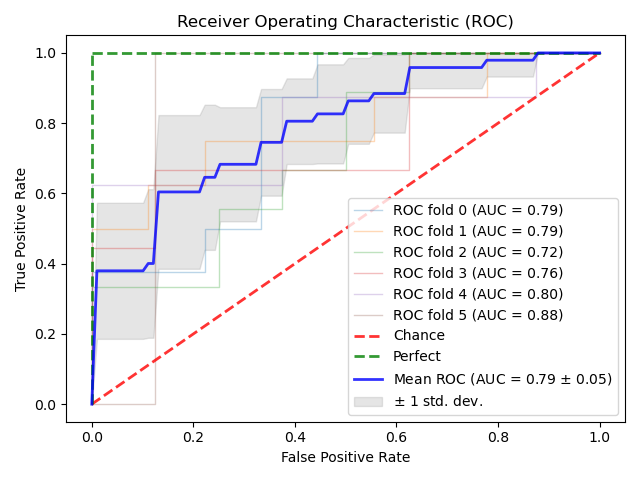
\includegraphics[width=\linewidth]{images/roc_auc.png}
  \caption{A ROC\textsubscript{AUC} graph.}
  \label{fig:roc}
\end{figure}

\clearpage
\section{Evaluation}

In this section, we evaluate the strengths and weakness of our solutions, reflecting upon the original research question: \textit{Can medium-term train delays be predicted?}.

\subsection{ETL}

Our approach to constructing a dataset was haphazard. Railways are a very complex subject matter, and with no expert at hand, this complexity was an intimidating prospect. 

While good repositories of knowledge exist, there was often little to be done in the face of obscure data save push on. A subject matter expert would have proved very helpful.

We did not appreciate how time-consuming the ETL task would be. It is industry knowledge that data preparation accounts for roughly $80\%$ of the work of a data scientist. 


It also took some time to settle on the research question. Was it better to tread the better-worn path of real-time delay prediction, and accept the enormous overhead of modelling a railway network, or to explore medium-term prediction? We chose medium-term prediction at a fairly late stage at the project, and as a result needless effort was expended ensuring the codebase was compatible with both timeframes. This is most obviously manifest in the movement dataset used. TRUST is briefly mentioned as an alternative, simpler, system to Darwin. However, using it would have precluded the use of forecasts. When investigating real-time delays, we discovered that a key performance indicator of any potential system is how predictions compare to the those made by the current system (in this case, Darwin). By the time we had chosen to explore medium-term delays, it was too late to revert back to TRUST, and more time was spent on comprehension.

As discussed previously, predicting primary delays is dependent on the inclusion of exogenous data. Many of the relevant categories were unfortunately unavailable in the archive used and so could not be included. As this dissertation progressed, a new repository, archiving all feeds, was established by OpenTrainTimes\footnote{https://networkrail.opendata.opentraintimes.com/}. However, switching would have incurred too much work, both from an extraction, but particularly a transformation, perspective, at a late stage of the project. We regrettably could not use several other important data sources. Infrastructure, in particularly, would have likely yielded far better performance.

Even the inclusion of weather was a challenge. The MIDAS dataset contained $192$ columns. Geolocating stations was problematic. As the project never developed to a working application, it proved unnecessary to convert MIDAS data to Datapoint data. We briefly mention earlier that 42\% of delays can be attributed to infrastructure faults. It is unfortunate that we were unable to include this data in our project. RF perform well quickly. It is normally possible, however, to create more complex models, such as Deep Neural Networks (DNNs) with superior performance. Using \verb|scikit-learn| proved to be a challenge, and introduced a sharp learning curve. These minor shortcomings in the planning of this project did not, owever, have an adverse effect on the quality of the solution produced. With few directly comparable studies, and no dataset, it is difficult to objectively state whether our solution is 'good'. 



\subsection{Binary classification}

Our approach to selecting a binary classification model proved sound. Initial early testing revealed that the class imbalance of our dataset seriously hampered performance, but this issue was neatly resolved a combination of resampling methods. The simple alternative approach, to balance the classes by discarding the an appropriate proportion of the majority, would have reduced the size of our dataset by $80\%$, with a corresponding decrease in model performance. Collecting more data might have made this viable; we chose a years' worth both to preserve the cyclical nature of the dataset and to limit resource consumption. At time of writing, approximately 2 years' worth of data is available online, and the codebase is written such that using this data is easy. 

The linear models performed poorly, as expected. We anticipated random forests and gradient-boosted decision trees to perform similiarly well, and indeed, though the former achieved the greatness recall and $F_1$-score, the latter achieved the best precision score. Random forests are, by nature, not easily fine-tuned. We identified only $4$ hyperparameters to modify, and though an exhaustive parameter optimisation yielded only a small improvement, we are satisfied with our model. 

Further investigation into feature importance revealed a number of features that contributed essentially nothing to performance. Random forest training time scales quadratically with the number of the features, so we pruned where necessary.

We anticipated datetime features being of most importance, and this was clearly the case - the top $15$ features are from datetime data. 

Considerable time was spent on train schedules in search of metadata that would enhance our dataset. Had we known how little some of these features contributed, our time could have been spent more profitably elsewhere. 

Extensive cross-validation revealed that our model was seriously overfitted, and so we removed a variety of features.

The main limitation of our model is the rigidity. 

While \verb|scikit-learn| is designed to be easy to use, we found that we pushed the API to its limits. We had particular trouble using \verb|scikit-learn| in conjunction with \verb|imbalanced-learn|.

\subsection{Hyperparameter optimisation}


\clearpage
\section{Conclusion}

In this project we have demonstrated how a novel, high-quality train delay dataset may be constructed from a variety of complex publicly available sources. To the best of our knowledge, this is the first time these sources have been utilised in this fashion.  

Using this dataset, we have produced two solutions to the problem of medium-term train delay prediction, one classification, the other regression. To achieve this, eight classifiers were tested and their performance evaluated. The most performant model, a random forest, was subject to further testing in which we systematically modified hyperparameters and encoding schemes to improve performance. Our final classification model achieved an accuracy of $50\%$ and an $ROC_{AUC}$ of $0.76$. We extended this solution to a regression model which achieves an \verb|MSE| of $1.0$. 

A suitable direction for future work would be the inclusion of more exogenous data, such as infrastructure, and a more complex model to better capture the secondary delays caused by interactions between trains. It is possible that alternative architectures such as Deep Neural Networks (DNN) would have yielded superior results to our random forest; this could be investigated. 

We discussed earlier that the main rationale behind this project the potential benefits it could yield for passengers. To make this project directly useful for consumers, a system could be developed that subscribes to real-time schedule and weather data to predict live whether a given train will be delayed, and, if so, by how much.  

\clearpage
\bibliography{projectpaper}


\end{document}